\documentclass[12pt]{toptesi}
\newif\ifpdf
\ifx\pdfoutput\undefined
   \pdffalse
\else
   \pdfoutput=1
   \pdftrue
\fi
\ifpdf
   \usepackage{graphicx}
   \usepackage{epstopdf}
   \DeclareGraphicsRule{.eps}{pdf}{.pdf}{`epstopdf #1}
   \pdfcompresslevel=9
\else
   \usepackage{graphicx}
\fi
\usepackage{wrapfig}
\usepackage{multirow}
%\usepackage{rotating}
\usepackage{booktabs}
\usepackage[utf8x]{inputenc}
\usepackage[superscript]{cite}
\usepackage{longtable}
\usepackage{amssymb}

%\usepackage{setspace}  % package per l'interlinea
%\onehalfspacing		% interlinea 1,5 con setspace

%\interlinea{1.3}		% interlinea di toptesi (è 1.3 perché 1.5 sembra davvero troppo) DECOMMENTARE prima della fine
						% sistemare tabella stadi puberali

\ateneo{Universit{\`a} degli Studi di Torino}
\facolta{Medicina e Chirurgia - Torino}
\logosede{logo}
\titolo{Impatto della terapia con ormone somatotropo sulla statura finale dei bambini nati piccoli per l'et\`a gestazionale}
\candidata{Sara Bertolotto}
\relatore{prof.ssa Barbara Stasiowska}
\sedutadilaurea{Marzo 2011}
\includeonly{%
preliminari,%
introduzione,%
scopo,%
casistica,%
risultati,%
conclusioni,%
nota39
}
\begin{document}
\frontespizio

%\sommario

%I risultati dell'applicazione della terapia con GH sui bambini nati piccoli per l'et\`a gestazionale sul territorio Piemontese.

%\tablespagetrue\figurespagetrue % normalmente questa riga non serve ed e' commentata
\indici

\large
\mainmatter

\chapter{Introduzione}
 
Il basso peso alla nascita \`e una delle maggiori cause di morbilit\`a e mortalit\`a
nel periodo neonatale e nell'infanzia in tutto il mondo.
Osservazioni epidemiologiche hanno evidenziato che i soggetti nati piccoli 
per l'et\`a gestazionale (SGA) presentano un aumentato rischio di 
alterazioni metaboliche e malattie cardiovascolari in età adulta\cite{consensus}.

Il 10-15\% dei bambini SGA è destinato a non raggiungere la statura normale\cite{karlberg1995growth} \cite{leger1997reduced}.

\section{Definizione di SGA}

In base ai dati antropometrici rilevati alla nascita, i neonati vengono classificati come:
\begin{itemize}
\item piccoli per l'epoca gestazionale (SGA - small for gestational age) quando presentano peso e/o lunghezza inferiori al 3°
   percentile o alle -2SD rispetto alle curve di normalità per sesso relative alla popolazione di appartenenza;
\item adeguati per l'epoca gestazionale (AGA - adeguate for gestational age) quando presentano peso e/o lunghezza compresi
   fra il 3° e il 90° percentile;
\item grandi per l'epoca gestazionale (LGA - large for gestational age) quando presentano peso e/o lunghezza superiori
   al 90° percentile\cite{sga-1}.
\end{itemize}

Da ciò emerge che è necessario conoscere l'età gestazionale e disporre di standard antropometrici di riferimento per la popolazione di appartenenza, così da stabilire correttamente quando peso e/o lunghezza si collochino al di sotto del 3° percentile o siano inferiori alle -2 DS.

 Occorre notare che la definizione SGA non considera alcuni fattori di fondo che modificano la crescita, come la taglia fisica della madre,
l'etnia e la gemellarit\`a\cite{consensus}.

L'acronimo SGA è spesso erroneamente considerato sinonimo di IUGR (Intrauterine Growth Retardation), pur non essendo i due termini
equivalenti: la definizione di IUGR è primariamente di tipo ostetrico, basata su due misurazioni ecografiche che evidenzino la ridotta crescita fetale.
Un neonato che ha presentato un ritardo di crescita intrauterino non necessariamente pu\`o essere classificato come uno SGA,viceversa un
neonato SGA pu\`o essere definito IUGR. Infatti un feto che presenta un rallentamento intrauterino della crescita può collocarsi dal punto di vista 
auxologico alla nascita anche sopra le -2 DS\cite{sga}.

\section{Prevalenza dei nati SGA}

Circa il 5\% dei nati in tutto il mondo sono piccoli per l'età gestazionale, 
ma questo dato è decisamente sottostimato: nei Paesi poveri in via di sviluppo 
e del terzo mondo i neonati spesso non vengono pesati e misurati\cite{novonordisk}.

Nella regione Piemonte nell'anno 2005 sono nati 36500 bambini (fonte ISTAT); di questi 800 (2,3\%) sono SGA. Una significativa percentuale di questi bambini (10\%, ovvero 80/anno) è destinata a rimanere di statura inferiore alla norma. Per confronto altre basse stature patologiche, come da deficit di GH e sindrome di Turner, presentano un'incidenza nettamente inferiore (deficit di GH 1/3500 nati, cioè 10/anno; s. di Turner 1/2500 nate, vale a dire 15/anno). L'incidenza di bassa statura in SGA è quindi otto volte superiore all'incidenza di bassa statura da deficit di GH e sindrome di Turner. 


\section{Cause}

Le cause del ritardo di crescita intrauterino si dividono in
fetali e materno -- placentari.


Tra le più frequenti cause fetali vi sono la gemellarità, le malformazioni congenite, le cromosomopatie e le sindromi dismorfiche: sindrome di Turner, sindrome di Cornelia de Lange, sindrome di Bloom, sindrome di Williams, trisomie dei cromosomi 13, 18, 21.

Altre cause genetiche comprendono le delezioni, le mutazioni, i polimorfismi dei geni codificanti per IGF-1, IGF-1R \cite{woods1996intrauterine} \cite{vaessen2002association} \cite{arends2002polymorphism}
e le disomie uniparentali materne dei cromosomi 14, 16, 20\cite{fowden2006imprinted}.
 
Per quanto concerne queste ultime, occorre considerare che, sebbene
i geni con imprinting non rappresentino oltre lo 0,5\% dell'intero genoma, essi svolgono
però un ruolo importante nel regolare lo sviluppo fetoplacentare, controllando l'accrescimento, la 
morfologia e la capacità di scambio di nutrienti tra la placenta e il feto.
In particolare il gene IGF-2 sembra essere fortemente coinvolto nella regolazione dello sviluppo
fetoplacentare. L'importanza dell'imprinting genico è dimostrata dall'effetto della disomia uniparentale
nell'uomo e nei roditori: l'accrescimento è stimolato dalle disomie paterne, mentre \`e inibito da quelle materne.\cite{fowden2006imprinted}.
Ad esempio il 10\% dei soggetti con sindrome di Silver Russell (condizione caratterizzata da IUGR, scarso accrescimento postnatale, asimmetria corporea e dismorfie facciali) presenta una disomia uniparentale materna del cromosoma 7. 

Infine Gicquel et al. in un recente studio hanno osservato che alterazioni epigenetiche del locus 11p15 (in particolare l'ipometilazione dell'Imprinting Control Region 1), che esitano nel silenziamento del gene dell'IGF-2, sono presenti nel 50\% dei soggetti con la sindrome di Silver Russell\cite{gicquel2005epimutation}.


Le cause materno -- placentari comprendono: le malattie croniche ed infettive, l'assunzione di farmaci, l'eccessivo carico di lavoro, il fumo, l'assunzione di sostanze stupefacenti, l'abuso alcolico e l'alimentazione inadeguata.

Fra le malattie croniche materne che compromettono l'accrescimento fetale vanno ricordate le cardiopatie, le patologie ematologiche, polmonari, metaboliche, renali ed autoimmuni. Per quanto riguarda le infezioni, esse rappresentano una delle più frequenti cause di iposviluppo fetale soprattutto nei paesi poveri e comprendono principalmente le infezioni appartenenti al gruppo TORCH (Toxoplasmosi, Rosolia, Citomegalovirus, Herpes Virus) e l'infezione da HIV.
Tra le cause materne vanno inclusi anche i farmaci assunti durante la gravidanza.In particolare sono da ricordare i chemioterapici, gli anticomiziali. Non vanno dimenticati gli agenti chimici, ad esempio alcuni solventi.

Bisogna considerare anche il tipo di attivit\`a lavorativa, con l'ammontare delle ore
che vi vengono dedicate durante la gestazione: in un recente studio Bonzini et al. hanno confermato che il lavoro pesante, 
richiedente un impegno fisico importante o uno sforzo prolungato, soprattutto se nell'ultimo trimestre,
può determinare parto pretermine, eclampsia, rottura prematura delle membrane e nascita di neonati IUGR e/o SGA\cite{sga-14}.

\`E molto importante sottolineare che la gravidanza è influenzata negativamente dal fumo di sigaretta in tutta la sua evoluzione.I metaboliti del tabacco agiscono creando
una situazione di ipossia fetale soprattutto tramite due meccanismi: la formazione di carbossi -- emoglobina, 
per legame tra emoglobina e monossido di carbonio; l'aumento della secrezione di catecolamine plasmatiche
dalla midollare del surrene, che causando vasocostrizione dell'arteria uterina e di quella ombelicale riducono l'afflusso ematico al feto.
Purtroppo si tratta di un problema non irrilevante, se si considera che le donne fumatrici in gravidanza costituiscono il 23,7\% delle gestanti (sondaggio ISTAT 2001).
Il Centro Internazionale di Consultazione sul fumo ha concluso che il tabagismo durante la gestazione \`e la maggiore causa di basso peso alla nascita\cite{sga-18}.
Dejin-Karlsson et al. hanno altres\`i verificato l'importanza del fumo passivo\cite{sga-20}. 

Recenti studi condotti da Stein e Chiaffarino hanno confermato che anche l'abuso di sostanze stupefacenti e/o di alcolici influenza negativamente la gravidanza comportando un maggior rischio di iposviluppo fetale\cite{sga-24}\cite{sga-25}.

La malnutrizione materna, spesso associata ad un basso stato socio--economico, rappresenta un'altra causa di scarso accrescimento intrauterino. 
Infatti, come \`e emerso da uno studio di Mitchell et al., le donne con figli AGA presentano una dieta più ricca in carboidrati, frutta, ferro ed acido folico rispetto a donne con figli SGA. In particolare gli autori hanno osservato che è soprattutto la supplementazione di acido folico già al momento del concepimento a ridurre il rischio di avere figli piccoli per l'età gestazionale, oltre che il rischio di mielomeningocele nel nascituro.\cite{sga-26}
Un recente studio condotto da Salvatore et al. riporta un rischio aumentato di presentare gravidanze complicate in donne con celiachia non diagnosticata: l'infiammazione del piccolo intestino causa uno
scarso assorbimento di sostanze nutritive e di conseguenza un quadro di malnutrizione materno--fetale\cite{sga-15}.

Tra le altre cause di iposviluppo fetale possiamo annoverare le differenze esistenti fra paesi in via di sviluppo e industrializzati.

Nei paesi in via di sviluppo le principali cause di dismaturità includono il fumo, l'inadeguato stato di 
nutrizione materna, la giovane età della gravida (parto prima dei 16 anni) nonché le infestazioni del Plasmodium della malaria a 
livello placentare.
\clearpage
Nei paesi industrializzati la nascità di bambini piccoli per l'età gestazionale
è spesso legata alla gemellarità (favorita da pratiche di fecondazione assistita
e dall'elevata età materna, superiore ai 35 anni), al fumo oppure alla dieta restrittiva e rigida della gestante.

\begin{table}[h]\centering
\begin{tabular}{cll}
\toprule
			& \multicolumn{1}{c}{Paesi sviluppati}			& \multicolumn{1}{c}{Paesi in via di sviluppo} \\
\midrule
Fetali & Gemellarit\`a  			& Infezioni			\\
 & (da fecondazione assistita) & \\\midrule
\multirow{4}{*}{Materno -- placentari} & Fumo						& Fumo/povertà		\\\cmidrule(l){2-3}
			& Dieta restrittiva e rigida	& Inadeguata nutrizione\\
			& &  materna \\\cmidrule(l){2-3}
			& Avanzata età materna  &	Giovane età materna \\\cmidrule(l){2-3}
			& Disfunzioni placentari	& Eccessivo carico di lavoro	\\\bottomrule
\end{tabular}
\label{tab-cause}
\caption{Cause di iposviluppo fetale in correlazione al paese di origine.}
\end{table}

Come vediamo i bambini SGA costituiscono un gruppo multiforme per eziologia.

Dal punto di vista clinico è importante una suddivisione che consideri la diversa compromissione delle principali variabili antropometriche: peso,lunghezza e circonferenza cranica.

La maggior parte degli individui SGA (80\%) presenta alla nascita il peso ridotto, ma la lunghezza e la circonferenza cranica sono normali o solo lievemente ridotti.
In questo caso la noxa (gestosi, malattie, malnutrizione materna) agisce piuttosto tardivamente, dopo la ventiseiesima settimana di gestazione e compromette soprattutto la biometria addominale: in condizioni di scarso afflusso sanguigno viene privilegiato lo sviluppo degli organi nobili (cervello, cuore, surrene) a scapito della massa epatica, che va incontro ad ipotrofia cellulare. 
Qusta situazone porta ad un ritardo di crescita disarmonico (SGA asimmetrico), con prevalente deficit ponderale.

Le cause fetali (in particolare le alterazioni genetiche e le sindromi cromosomiche) o l'insufficienza utero-placentare severa ad esordio 
precoce, vale a dire prima della sedicesima settimana di gestazione,oltre a gravi infezioni materne, farmaci e fumo  hanno un impatto pi\'u importante sullo sviluppo fetale, comportando un'ipocellularità con riduzione sia della circonferenza addominale, che della lunghezza degli arti e della circonferenza cranica. In tal caso si parla di SGA simmetrico, altrimenti detto "`low profile"' o armonico, caratterizzato da ridotta lunghezza, deficit ponderale e circonferenza cranica inferiore alla norma (20\% dei bambini SGA).

La distinzione fra SGA asimmetrici e simmetrici \`e importante: Albertsson--Wikland et al. hanno osservato che i bambini con deficit prevalentemente ponderale alla nascita 
(SGA asimmetrici) presentano una migliore prognosi staturale rispetto agli SGA simmetrici.\cite{sga-10}

\clearpage

\section{Complicanze}

I nati SGA presentano oltre alla bassa statura anche alterazioni endocrino--metaboliche e cardiovascolari. 
Per spiegare tali complicanze è stato proposto il modello del fenotipo risparmiatore (\textit{Thrifty phenotype}).
Secondo questa ipotesi, la malnutrizione intrauterina sarebbe il fattore scatenante
per innescare nel feto una serie di meccanismi di adattamento indispensabili per 
la sua sopravvivenza a breve termine, ma che comportano delle modificazioni permanenti
del metabolismo energetico.
Tali meccanismi di adattamento avvengono per favorire lo sviluppo dei tessuti 
nobili come quello nervoso, cardiaco e renale, a scapito dei tessuti adiposo ed endoteliale .

In particolare sembrerebbe instaurarsi una insulino--resistenza 
a livello periferico che, causando il calo della glicogenesi e della lipogenesi,
permette di mantenere i livelli plasmatici di glucosio e acidi grassi liberi
indispensabili per un corretto sviluppo del sistema nervoso e degli organi splacnici.\cite{sga-51}



\`E possibile distinguere conseguenze a breve e lungo termine che tale risposta
adattativa produce nei soggetti coinvolti.

Tra le ripercussioni immediate la più importante riguarda lo scarso accrescimento
staturo-ponderale presente sia a livello intrauterino che post nascita. Inoltre 
il nato piccolo per l'età gestazionale tende ad accumulare grasso in depositi a livello
viscerale a discapito di una corretta formazione di massa magra. Infine in un ambiente intrauterino non ottimale per l'accrescimento spesso il feto ricerca un tempo gestazionale
rapido (prematurità) \cite{sga-53}. 

Successivamente soprattutto nelle bambine si possono manifestare pubarca precoce e pubertà anticipata e/o a rapida progressione. 

Le conseguenze a lungo termine comprendono malattie della sfera glicometabolica (ridotta sensibilità insulinica,
ipertensione arteriosa, sovrappeso e obesità, diabete mellito) secondarie all'alterato sviluppo dei tessuti pancreatico, endoteliale ed adiposo.\cite{sga-32}


\section{Crescita nei bambini SGA: storia naturale}

Le misure alla nascita sono determinate principalmente dalle condizioni ambientali in utero. Successivamente, nei primi 12-18 mesi di vita extra-uterina, le differenze in peso e lunghezza determinate dalle condizioni prenatali si riducono, mentre aumenta la variabilità legata al patrimonio genetico. Pertanto in questo periodo gli individui nati piccoli da genitori di alta statura tendono a crescere di più, mentre quelli nati grandi da genitori di bassa statura tendono a crescere meno. 


La velocità di crescita è molto alta subito dopo la nascita: nei maschi la lunghezza aumenta nei primi 3 mesi ad una velocità di circa 40 cm/anno; successivamente questa velocità diminuisce gradualmente raggiungendo i 14 cm/anno fra l'età di 9 mesi e 1 anno. La velocità di crescita ponderale presenta il proprio picco fra il primo e il secondo mese di vita dopo la nascita, poi segue una graduale riduzione; così la velocità iniziale di circa 10 kg/anno scende a 3 kg/anno tra l'età di 9 e 12 mesi. Tra l'età di 2 e 4-5 anni la velocità di crescita staturale diminuisce progressivamente\cite{tanner1994growth}.
 All'età di 5 anni il bambino entra in una fase di latenza. In questo periodo la statura aumenta di circa 5 cm/anno. In pubertà il corpo incomincia a crescere ad alta velocità e la statura aumenta di 10 cm nell'anno centrale di scatto puberale per i maschi e di 8 cm per le femmine. Si tratta di velocità comunque inferiori rispetto a quelle riscontrabili nei primi due anni di vita.
 La figura 1.1 illustra l'andamento di crescita nei diversi periodi di vita evolutiva.
 
\begin{figure}[!h]
  \begin{center}
      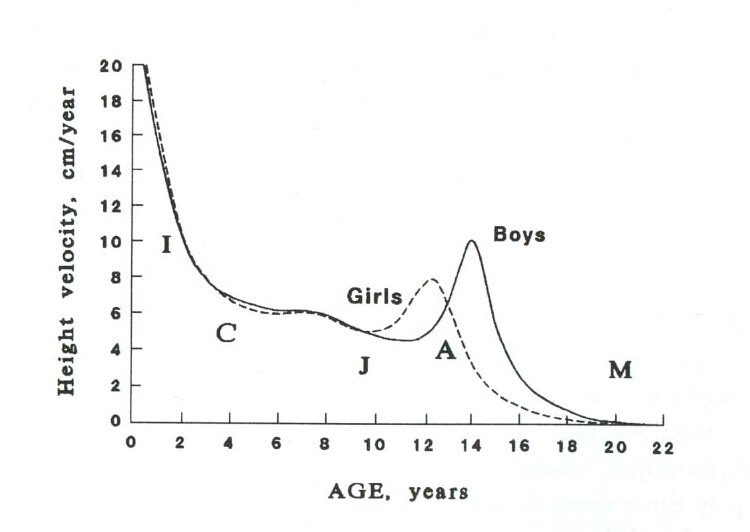
\includegraphics[scale=0.85]{grafici/grafico_velocita} %\\
  \end{center}
  \caption{Curve di velocità di crescita staturale per maschi e fammine sani.\\I: prima infanzia, C: seconda infanzia, J: terza infanzia, A: pubertà, M: età adulta. \cite{bogin1996evolution} }
  \label{fig:GraficoVelocita}
\end{figure}
 
I bambini con deficit di crescita intrauterino nella grande maggioranza dei casi presentano crescita di recupero(\textit{catch up growth}), la quale è un accrescimento superiore al normale che segue un periodo di restrizione e che compenserà, almeno in parte, il deficit di crescita causato da condizioni patologiche \cite{boersma1997catch}.
La crescita di recupero è attesa, ad esempio, dopo la correzione di deficit di GH, malnutrizione, malattia celiaca o ipotiroidismo. I meccanismi che si celano dietro questa crescita compensatoria non sono chiari, ma studi sperimentali sulla restrizione di crescita suggeriscono che un temporaneo arresto della senescenza dei condrociti della cartilagine di accrescimento potrebbe essere uno dei meccanismi 
coinvolti.
La teoria si basa sull'ipotesi che la cartilagine di accrescimento abbia una sua storia replicativa, assumendo un limite alla capacità proliferativa dei condrociti. Una temporanea condizione avversa, rallentando il tasso di crescita dei condrociti, ne postporrebbe la senescenza.\cite{gafni2001catch} 


Considerata la dinamica della crescita staturale esposta in precedenza, la crescita di recupero ha più successo nei primi due anni di vita, come in realtà avviene nel 90\% dei nati SGA\cite{karlberg1995growth}. Ciò permette loro di raggiungere una statura normale, ma non necessariamente media. Infatti la statura media degli adulti nati SGA è di circa 1 DS al di sotto della statura 
media della popolazione generale\cite{leger1997reduced}. Secondo i centili italiani di riferimento \cite{cacciari2006italian} la statura media della popolazione generale corrisponde a 163 cm per le femmine ed a 176 cm per i maschi. Considerando che la statura media dei nati SGA è 1 DS inferiore rispetto alla statura media della popolazione generale,   
si ottiene che la statura media per un individuo italiano nato SGA è di 157 cm per le femmine e di 170 cm per i maschi. 


Il 10\% degli individui nati SGA non raggiunge la statura normale, cioè presenta una statura finale inferiore alle -2 DS, vale a dire al di sotto dei 151 cm per le femmine ed inferiore ai 164 cm per i maschi. 
Le cause di bassa statura nei soggetti SGA comprendono: mancata o incompleta crescita di recupero; pubertà sovente anticipata e a rapida progressione; scatto puberale di crescita ridotto; maturazione scheletrica inizialmente ritardata seguita da rapida accelerazione. Infine una certa percentuale di bambini SGA presenta un'insufficiente produzione di ormone della crescita\cite{leger1997reduced}.
 

La crescita di recupero è assente o incompleta negli individui nati SGA per lunghezza. In particolare è stato stimato che il rischio relativo di bassa statura all'età di 18 anni tra i bambini nati SGA è 5,2 per quelli 
piccoli in peso e 7,1 per quelli piccoli in lunghezza. \cite{cianfarani2006hormonal}. Anche l'eventuale presenza di un quadro sindromico (ad esempio la sindrome di Silver Russell) riduce le probabilità di recupero staturale. Un'altra importante variabile che condiziona la crescita di recupero è la statura dei genitori: i bambini SGA nati da genitori bassi generalmente non presentano un soddisfacente recupero staturale. Anche la grave prematurità, così come le anomalie genetiche/i polimorfismi dell'asse GH--IGF-1 influenzano negativamente la crescita di recupero. 


Un'altra causa di bassa statura nei soggetti nati SGA è la pubertà sovente anticipata e/o a rapida progressione\cite{albertsson2000children}.
Come evidenziato dagli studi osservazionali di Prader\cite{gasser1985human}, Stanhope\cite{stanhope1988new}
e Largo \cite{gasser2001growth} 
 la statura finale dipende prevalentemente dalla velocità di crescita prepuberale nei maschi, nelle femmine anche dalla durata di crescita prepuberale: è stato stimato che all'ingresso in pubertà le ragazze hanno già realizzato circa l'85\% ed i ragazzi circa il 90\% della statura definitiva . Inoltre il guadagno in statura che si ottiene durante lo scatto puberale è legato più alla durata dello scatto,che alla sua intensità. Ciò significa che se l'individuo anticipa la pubertà sottrae tempo alla crescita prepuberale e dunque centimetri significativi per la sua statura finale. Se inoltre la pubertà del soggetto è a rapida progressione viene meno l'ultima possibilità per migliorare la statura definitiva, poichè viene ridotta la durata dello scatto puberale.
 

Per quanto concerne la maturazione scheletrica, i bambini SGA tendono ad avere un'età ossea modicamente ritardata (anche di due anni) fino all'epoca puberale, dunque una previsione della statura definitiva basata sull'età ossea e fatta in età prepuberale potrebbe fornire risultati rassicuranti. Tuttavia l'inizio anticipato della pubertà e la successiva accelerazione dello sviluppo puberale associato a rapida maturazione scheletrica determinano un crollo della previsione e, sopratutto, della effettiva statura finale\cite{job1986histoire}.

Il raggiungimento di una statura inferiore alla norma (vale a dire al di sotto di -2DS)è un evento più comune nella popolazione nata SGA che negli individui con peso alla nascita adeguato, come dimostrato da uno studio a lungo termine condotto da Leger et al. su 213 soggetti SGA e 272 con peso alla nascita normale. Questo studio ha evidenziato che il 
13,6\% degli individui nati SGA presentava una statura inferiore a -2 DS all'età di
20-21 anni, contro solo l'1.8\% del gruppo di controllo.\cite{leger1997reduced}

I soggetti nati SGA costituiscono una componente importante degli adulti di bassa statura (25\%) e rappresentano una popolazione destinata ad aumentare numericamente se si considerano i fattori di rischio per la nascita di bambini SGA .

Va notato che una bassa statura persistente può associarsi ad una significativa alterazione degli aspetti psico-sociali.\cite{kelnar1990pride} In particolare un recente studio condotto sulla popolazione generale del Regno Unito ha dimostrato l'impatto negativo che una bassa statura può esercitare sulla qualità della vita, intesa come benessere fisico, psicologico e sociale\cite{christensen2007evaluation}. 

 \chapter{Scopo della ricerca}

\section{Premesse: la terapia con GH nei bambini SGA}


Il GH ("growth hormone", ormone della crescita) agisce a livello di diversi organi e apparati.
L'azione principale nell'infanzia e nell'adolescenza si esplica attraverso l'accrescimento
longitudinale delle ossa, stimolando la proliferazione e la differenziazione dei condrociti
a livello delle cartilagini di accrescimento epifisarie con successiva calcificazione
e incorporazione nell'osso metafisario. Esso stimola inoltre la sintesi del collagene 
di tipo I e la proliferazione osteoblastica.\cite{sga}


Nonostante non fosse ancora chiara l'eziologia della bassa statura nei soggetti SGA,
negli anni '70 si è iniziato l'approccio terapeutico con l'ormone della crescita.

In particolare nel 1969 vennero trattati per la prima volta con ormone della crescita  due bambini nati piccoli per l'età gestazionale affetti dalla sindrome di Silver Russell. Durante il trattamento i due pazienti mostrarono un significativo aumento della velocità di crescita staturale e si avvicinarono al terzo centile delle carte staturali di distanza. Purtroppo non furono riportati i dati sulla statura finale.%citare nota bilio 64 del consensus

Nel 1974 furono trattati con GH otto bambini con ritardo di crescita intrauterino. Anche in questo studio venne riportato un incremento della velocità di crescita degno di nota durante la terapia.% citare nota bilio 65 del consensus


Visti gli incoraggianti risultati a breve termine e notando che altri pazienti senza deficit di GH traevano beneficio dalla terapia con ormone somatotropo (ad esempio le bambine con sindrome di Turner)%citare nota bilio auxology pag 352(Betts),
si proseguirono gli studi sui bambini SGA in trattamento con GH.


Nel 2009 è stata effettuata una meta-analisi di ventinove studi su bambini SGA. Di questi solamente quattro sono stati considerati validi in termini di durata della terapia (superiore ad un anno), continuità della stessa ed obiettivo (impatto della terapia sulla statura finale).% citare Arianna Maiorana e Stefano Cianfarani (2009); togliere dalla bibliografia, almeno temporaneamente, tutti gli altri articoli riassunti sotto

Dunque finora pochissimi studi hanno valutato l'effettivo impatto della terapia continua e di lunga durata con rGH sulla statura finale dei bambini nati SGA . 






%Inizialmente i risultati non furono brillanti, probabilmente per il trattamento non 
%ottimale in termini di dosaggio e frequenza di somministrazione. Nonostante ciò i 
%bambini SGA trattati con l'ormone somatotropo per due, tre anni crescevano meglio
%rispetto a quelli non trattati. Sulla base di tali osservazioni si è proseguito con
%il trattamento, modificandone il dosaggio e la frequenza di somministrazione.
 

%Gli studi condotti negli ultimi 30 anni hanno permesso di verificare l'efficacia,
%l'utilit{\`a}, la sicurezza e soprattutto l'adeguatezza della dose dell'ormone somatotropo
%nei bambini nati piccoli per l'et{\`a} gestazionale.


%In particolare:

%\begin{description}
%\item[Anita Hokken-Koelega et al. (2003)] \hfill \\
%si tratta di uno studio multicentrico che ha preso in considerazione 165 bambini SGA prepuberi.75 di questi sono stati assegnati casualmente alla valutazione della risposta al trattamento con ormone della crescita biosintetico alla dose di 0.033 mg/kg/die (gruppo A,n=41) e alla dose di 0.067 mg/kg/die (gruppo B, n=38). I restanti 90 bambini sono stati casualmente sottoposti ad una dose di GH pari a 0.033 mg/kg/die (n=60) o destinati al gruppo di controllo (n=30). Scopo dello studio era valutare gli effetti della terapia con GH su composizione corporea, metabolismo dei carboidrati e altezza finale nei soggetti SGA.Lo studio è durato 6 anni, al termine dei quali è emerso che la terapia con GH per lungo periodo e senza interruzioni porta alla normalizzazione della statura nell'infanzia e ad una normale statura finale nella maggior parte dei bambini, indipendentemente dalla dose. Solo bambini molto bassi o di età maggiore necessitano di dosaggi alti. Inoltre si è dimostrato che la terapia con GH non ha effetti avversi sui livelli di glucosio e sui lipidi sierici ed ha un effetto positivo sulla pressione arteriosa. Tuttavia il GH induce un innalzamento dei livelli  di insulina, segno di insulino-resistenza; i livelli di insulina tornano nell'intervallo di normalità con la cessazione della terapia. Infine si è visto che la terapia con GH migliora significativamente la mineralizzazione ossea e la massa magra dei bambini nati SGA. 

%\item[Yvonne Van Pareren et al. (2003)] \hfill \\
 %questo studio multicentrico si è posto come obiettivo la valutazione dell'effetto di un trattamento continuo ed a lungo termine con GH sulla statura finale di 54 bambini bassi nati SGA.I bambini,alcuni dei quali risultati parzialmente  deficitari di GH, sono stati suddivisi casualmente in due gruppi: uno trattato con GH alla dose di 3 UI (0.033 mg/kg/die); l'altro trattato con una dose maggiore (6 UI = 0.067 mg/kg/die). Il trattamento è durato circa 2 anni. Come controllo si è scelto un gruppo di bambini nati SGA non deficitari di GH i cui pediatri si sono opposti al trattamento ormonale. Si è osservato che, indipendentemente dalla produzione di GH prima del trattamento e a prescindere dalla dose assunta nel corso del trattamento, la maggior parte dei bambini ha raggiunto una statura finale compresa nell'intervallo di normalità e la quasi totalità 
% ha raggiunto una statura entro i limiti del bersaglio parentale. Solo bambini SGA estremamente bassi o con centro target al di sotto dell' intervallo di normalità potrebbero necessitare di alte dosi di ormone della crescita. Gli autori concludono dicendo che sono necessari ulteriori studi per ottimizzare il trattamento con GH dei bambini SGA al fine di individuare la migliore opzione terapeutica per ogni bambino. 

%\item[Myriam Rosilio et al. (2005)] \hfill \\
 %si tratta di uno studio multicentrico condotto su 35 bambini prepuberi nati SGA. I bambini hanno ricevuto quotidianamente per due anni una dose di ormone delle crescita biosintetico piuttosto alta (0.067 mg/kg/die). Alcuni di questi bambini hanno riassunto l'ormone dopo una pausa di 2 anni. Non sono emerse alterazioni riguardo al metabolismo del glucosio durante il trattamento e nel successivo follow-up. è stata riportata l'altezza finale di 20 dei 35 soggetti inclusi nello studio. I modesti risultai ottenuti in termini di SDS guadagnate sono probabilmente attribuibili alla breve durata del trattamento ed al suo schema discontinuo. Gli autori affermano che ulteriori studi sono necessari per chiarire la risposta al trattamento ed individualizzarlo.

%\item[Arianna Maiorana e Stefano Cianfarani (2009)] \hfill \\
 %è una meta-analisi di 29 studi su bambini SGA. Di questi solamente quattro vengono considerati validi in termini di durata della terapia (superiore ai due anni), continuità della stessa ed obiettivo ( impatto della terapia sulla statura finale).  Da questi quattro studi  emerge che la terapia con GH sembra essere efficace nel ridurre almeno in parte il deficit staturale che i soggetti SGA presentano in età adulta, senza differenze statisticamente significative fra i due regimi di dosi terapeutiche (0.033 vs 0.067 mg/kg/die). Gli autori concludono però che la risposta alla terapia è altamente variabile ed occorrono ulteriori studi per identificare coloro che rispondono alla terapia con un significativo miglioramento della statura finale.  

%\end{description}

%\nocite{hokken2003final,van2003adult,rosilio2005adult,maiorana2009impact}

%Da quanto esposto sopra emerge che :
%\begin{itemize}
%\item la terapia con GH non induce diabete nei soggetti nati SGA, i quali rappresentano una poplazione a rischio di complicanze glicometaboliche.
%\item attualmente gli studi valutanti l'impatto di una terapia continua e di lunga durata 
%con ormone somatotropo biosintetico sulla statura finale di bambini nati piccoli per l'età gestazionale sono pochi.
%\end{itemize}

 
 


%In Italia è possibile la prescrizione a carico del Servizio Sanitario Nazionale,
%secondo le direttive pubblicate sulla Gazzetta Ufficiale del 13 ottobre 2009 che 
%attraverso la Nota 39 ha uniformato sul territtorio nazionale le condizioni 
%richieste dalle Commissioni Regionali preposte per l'autorizzazione al trattamento.(in casistica)



\section{Obbiettivi dello studio}

Lo scopo del presente studio è presentare i risultati della terapia continua e a lungo termine  con GH biosintetico sulla statura finale dei soggetti nati piccoli per l'età gestazionale.

In particolare vengono considerati:

\begin{itemize}
\item l'altezza finale (final height, FH) espressa in Standard Deviation Score;
\item le SDS guadagnate, confrontando l'altezza finale in SDS con l'altezza all'inzio del trattamento espressa anch'essa in SDS;
\item l'altezza finale espressa in SDS e le SDS guadagnate corrette per il centro del bersaglio parentale (midparental height).
\end{itemize}




\chapter{Casistica, materiali e metodi}

\section{Casistica}

Introduzione alle informazioni della mostrate

\subsection{Paziente 1} % Ma.Va.

Breve descrizione ...

\begin{table}
\begin{tabular}{ll ll}
\toprule
\multicolumn{4}{l}{\textbf{Dati alla nascita}}\\
Luogo 		& Torino 	& Data 					& 28/12/89 (89.989)\\
Sesso 		& Femmina 	& Età gestazionale 		& 40 sett.\\
Lunghezza 	& 45 cm 	& Circonferenza cranica	& 35 cm\\
Peso 		& 3350 g\\
\midrule
\multicolumn{4}{l}{\textbf{Statura dei genitori}}\\
Padre 		& 165.5 cm 	& Madre 				& 164.2 cm \\
MPH 		& ?? \\
\midrule
\multicolumn{4}{l}{\textbf{Trattamento con GH}} \\
Età	iniziale	& ?? 		& Altezza iniziale 				& 135.5 cm  \\
Peso iniziale	& 25.4 kg	& Velocità di crescita iniziale & 4.13 cm/aa\\
Dose media		& ?? 		& Anni prepuberali trattati		& ??\\
Anni di terapia & ??\\
\midrule
\multicolumn{4}{l}{\textbf{Esito della terapia}} \\
Altezza finale	& ?? cm (?? SDS) & SDS guadagnate 			& ??\\
SDS per MPH		& ??			 & SDS guadagnate per MPH	& ??
\bottomrule
\end{tabular}
\end{table}

\section{Materiali e metodi}

\subsection{Valutazione auxologica}

\begin{figure}[h]
  \begin{center}
      \includegraphics{grafici/centili/centili.eps} %\\
  \end{center}
  \caption{Standard antropometrici neonatali relativi a peso ed altezza nell'Italia nord-orientale}
\end{figure}

\begin{figure}[h]
  \begin{center}
	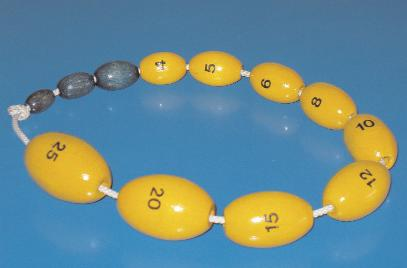
\includegraphics[scale=0.75]{grafici/orchidometro.jpg}
  \end{center}
  \caption{Orchidometro di Prader}
\end{figure}

\begin{figure}[h]
  \begin{center}
	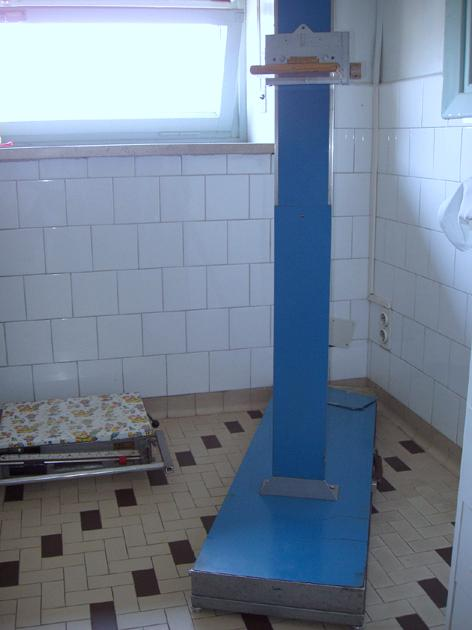
\includegraphics[scale=0.50]{grafici/statimetro.jpg}
  \end{center}
  \caption{Statimetro di Harpenden}
\end{figure}

\subsection{Valutazione ormonale}

\subsection{Analisi statistiche}

\chapter{Risultati}

\begin{table}[!h]
\begin{center}
\addtolength{\tabcolsep}{12pt}
\renewcommand{\arraystretch}{1.1}
\begin{tabular}{lcccc}
\toprule

 & Padre & Madre & MPH & SDS del MPH \\
% riga unità di misura
 & \emph{cm} & \emph{cm} & \emph{cm} & \\
\midrule
A.A.	& 170,6 & 160,4 & 159,0 & -0,5  \\
B.A.	& 170,1 & 156,8 & 156,9 & -0,9  \\
B.M.	& --    & --    & --    & --    \\
C.D.	& 157,7 & 147,8 & 159,2 & -2,3  \\
C.B.	& 165,7 & 161,2 & 156,9 & -0,9  \\
DL.V.	& 159,2 & 149,8 & 148,0 & -2,4  \\
D.A.	& 157,0 & 143,0 & 156,5 & -2,7  \\
DN.S.	& 154,8 & 155,9 & 148,8 & -2,3  \\
E.A.	& 144,5 & 139,2 & 148,3 & -3,9  \\
G.A.	& 168,2 & 137,2 & 146,2 & -2,7  \\
K.E.	&  &  &  &  \\            
L.A.	& 160,4 & 147,1 & 160,2 & -2,1  \\
L.R.	& 163,3 & 145,6 & 160,9 & -2,0  \\
L.L.	& 164,0 & 143,0 & 160,0 & -2,2  \\
M.V.	& 165,5 & 164,2 & 158,3 & -0,6  \\
M.E.	& 163,2 & 142,6 & 146,4 & -2,7  \\
P.G.	& 160,6 & 159,4 & 153,5 & -1,5  \\
P.D.	& 174,2 & 151,8 & 169,5 & -0,8  \\
P.C.	& --    & --    & --    & --    \\
P.S.	& 180,0 & 171,0 & 169,0 & 1,2   \\
R.M.	& 174,5 & 177,1 & 182,3 & 1,1   \\
S.M.	& 172,8 & 143,1 & 151,4 & -1,8  \\
S.F.	& 158,0 & 139,8 & 142,4 & -3,4  \\
S.A.	& 174,7 & 153,5 & 157,6 & -0,8  \\
V.D.	& 171,2 & 146,3 & 165,2 & -1,4  \\
Z.G.	& 165,5 & 150,0 & 151,2 & -3,4  \\
Z.M.	& 166,0 & 156,8 & 167,9 & -1,0  \\
Z.L.	& 161,4 & 146,1 & 160,2 & -2,1  \\
\bottomrule
\end{tabular}
\end{center}
\caption{Target genetico della popolazione in esame (con MPH e relativo standard score).}
\label{tab:TargetGenetici}
\end{table}

\begin{table}[!h]
\begin{center}
%\addtolength{\tabcolsep}{5pt}
%\renewcommand{\arraystretch}{1.1}
\begin{tabular}{lcccccc}
\toprule
 & \multirow{2}{*}{Sesso} & \multirow{2}{*}{Deficit GH} & \multicolumn{3}{c}{Altezza} & \multicolumn{1}{c}{Velocità di crescita} \\
 \cmidrule(r){4-6}
 & &   							& cm    & Centile  & SDS & cm/aa	 \\
\midrule
A.A.	& F &  				 		& 123,3 & $<$3  & -2,6 & 4,8 \\
B.A.	& F & \checkmark 	  				& 103,7 & $<$3  & -2,7 & 4,6  \\
B.M.	& F & \checkmark 	  				&  97,6 & $<$3  & -3,7 & 5,4 \\
C.D.	& M & \checkmark 	  				& 116,1 & $<$3  & -3,4 & 3,7 \\
C.B.	& F &  				 	        & 125,9 & $<$3  & -2,5 & 5,4 \\
DL.V.	& F & \checkmark 	  				& 109,5 & $<$3  & -2,5 & 6,0  \\
D.A.	& M &  				  		& 120,2 & $<$3  & -2,7 & 3,9 \\
DN.S.	& F & \checkmark 	  				& 122,8 & $<$3  & -3,6 & 5,2 \\
E.A.	& M &  				  		& 113,7 & $<$3  & -4,6 & 3,0 \\
G.A.	& F &  				  		&  88,1 & $<$3  & -3,2 & 5,5 \\
K.E.	& F &  				  		&       &       &      &     \\
L.A.	& M & \checkmark 	  				& 128,2 & $<$3  & -3   & 2,8 \\
L.R.	& M &  				  		& 117,7 & $<$3  & -2,9 & 3,6 \\
L.L.	& M &  				  		& 136,8 & $<$3  & -2   & 3,7  \\
M.V.	& F & \checkmark 	  				& 135,5 & $<$3  & -2,7 & 4,1 \\
M.E.	& F &  				  		& 122,6 & $<$3  & -4,8 & 3,7 \\
P.G.	& F & \checkmark 	  				& 121,7 & $<$3  & -2,9 & 2,5 \\
P.D.	& M &  				  		& 121,5 & $<$3  & -2,3 & 6,1 \\
P.C.	& F &  				  		& 105,8 & $<$3  & -2,8 & 4,9  \\
P.S.	& F &  				  		& 132,5 & $<$3  & -3   & --  \\
R.M.	& M & \checkmark 	  				& 112,2 & $<$3  & -3,1 & 5,0 \\
S.M.	& F & \checkmark 	  				& 122,0 & $<$3  & -2,2 & 4,0 \\
S.F.	& F &  				  		& 111,6 & $<$3  & -2,8 & 4,0 \\
S.A.	& F &  				  		& 120,8 & $<$3  & -2,8 & 5,4 \\
V.D.	& M &  				  		& 149,8 & 3--10 & -1,5 & 7,9 \\
Z.G.	& M &  				  		& 156,0 & 3     & -2   & 6,9  \\
Z.M.	& M &  				  		& 116,9 & $<$3  & -2,2 & 4,0 \\
Z.L.	& M &  				  		& 120,1 & $<$3  & -2,8 & 3,5 \\
\bottomrule
\end{tabular}
\end{center}
\caption{Situazione iniziale.}
\label{tab:SituazioneIniziale}
\end{table}


\begin{table}[!h]
\begin{center}
%\addtolength{\tabcolsep}{-1pt}
%\renewcommand{\arraystretch}{1.1}
\begin{tabular}{lcrcccl}
\toprule
 &      Sesso &   Età inizio  & Dose media 	& Anni prepuberali & Durata \\
 &     &				  & \emph{mg/kg/sett}	& & \emph{aa} \\
\midrule
A.A.	& F & 10,573  	      &  		    &              &     \\
B.A.	& F & 6,608   	      &             &                &     \\
B.M.	& F & 6,372   	      & 0,30        &              & 7,6 \\
C.D.	& M & 9,740   	      &             &                &     \\
C.B.	& F & 10,661  	      & 0,25        & 2,0                & 3,5 \\
DL.V.	& F & 7,499   	      &             &                  &     \\
D.A.	& M & 9,923   	      &             &                  &     \\
DN.S.	& F & 11,463  	      &             &                  &     \\
E.A.	& M & 10,849  	      &             &                  &     \\
G.A.	& F & 4,036   	      &             &                  &     \\
K.E.	& F &         	      &             &                  &     \\
L.A.	& M & 12,011  	      &             &                  &     \\
L.R.	& M & 9,589   	      &             &                  &     \\
L.L.	& M & 12,684  	      &             &                  &     \\
M.V.	& F & 12,283  	      &  0,26       & 2,5              & 3,6 \\
M.E.	& F & 11,559  	      &  0,33       & 3,5              & 4   \\
P.G.	& F & 10,272  	      &  0,26       & 2,5              & 4,6 \\
P.D.	& M & 9,602   	      &             &                  &     \\
P.C.	& F & 7,460   	      &             &                  &     \\
P.S.	& F & 11,997  	      &             &                  &     \\
R.M.	& M & 6,918   	      &             &                  &     \\
S.M.	& F & 9,719   	      &  0,27       & 2,6              & 4,7 \\
S.F.	& F & 8,313   	      &  0,26       & 3,5              & 6,0 \\
S.A.	& F & 10,079  	      &             &                  &     \\
V.D.	& M & 13,929  	      &             &                  &     \\
Z.G.	& M & 14,964  	      &  0,26       & 0                & 1,5 \\
Z.M.	& M & 8,507   	      &             &                  &     \\
Z.L.	& M & 9,877   	      &  0,28       & 3,5              & 5,5 \\
\bottomrule
\end{tabular}
\end{center}
\caption{Terapia.}
\label{tab:Terapia}
\end{table}


\begin{table}[!h]
\begin{center}
%\addtolength{\tabcolsep}{12pt}
%\renewcommand{\arraystretch}{1.1}
\begin{tabular}{lcrlc}
\toprule
 & Sesso 	& Età inizio pubertà	& Altezza	& Terapia frenante \\
 & &  \multicolumn{1}{c}{\emph{aa}} 	& \multicolumn{1}{c}{\emph{cm}}			\\
\midrule
A.A.	& F 	& 10,154 		& 121,8  		& \checkmark \\
B.A.	& F 	& 12,687 		& 137,9   		&            \\
B.M.	& F 	& 13,306 		& 141,5   		&            \\
C.D.	& M 	& 12,781 		& 136,2   		&            \\
C.B.	& F 	& 10,542 		& 125,0   		& \checkmark \\
DL.V.	& F 	& 11,104 		& 131,0   		&            \\
D.A.	& M 	& 10,405 		& 123,6   		& \checkmark \\
DN.S.	& F 	& 11,959 		& 126,3   		&            \\
E.A.	& M 	& 13,290 		& 125,7   		&            \\
G.A.	& F 	& 9,548  		& 122,5   		&            \\
K.E.	& F 	&        		&    		&            \\
L.A.	& M 	& 13,501 		& 134,3   		&            \\
L.R.	& M 	& 11,132 		& 127,5   		&            \\
L.L.	& M 	& 14,205 		& 146,6   		&            \\
M.V.	& F 	& 12,767 		& 139,3   		&            \\
M.E.	& F 	& 12,060 		& 126,8   		&            \\
P.G.	& F 	& 10,014 		& 121,1   		& \checkmark \\
P.D.	& M 	& 11,463 		& 132,9   		&            \\
P.C.	& F 	& 9,880  		& 123,8   		& \checkmark \\
P.S.	& F 	& 12,953 		& 140,0   		&            \\
R.M.	& M 	& 9,926  		& 135,6   		& \checkmark \\
S.M.	& F 	& 10,329 		& 126,8   		& \checkmark \\
S.F.	& F 	& 9,787  		& 124,1   		&            \\
S.A.	& F 	& 12,038 		& 137,8   		&            \\
V.D.	& M 	& 11,661 		& 138,4   		&            \\
Z.G.	& M 	&   --   		&    		&            \\
Z.M.	& M 	& 13,009 		& 139,5   		&            \\
Z.L.	& M 	& 11,874 		& 132,6   		&            \\
\bottomrule
\end{tabular}
\end{center}
\caption{Pubertà.}
\label{tab:Puberta}
\end{table}


\begin{table}[!h]
\begin{center}
%\addtolength{\tabcolsep}{12pt}
%\renewcommand{\arraystretch}{1.1}
\begin{tabular}{llcrrr}
\toprule
 & \multicolumn{2}{c}{Altezza finale} 	& SDS dal MPH	& SDS guadagnate & Scatto puberale \\
\cmidrule(r){2-3}
  & \emph{cm} 	& \emph{SDS}  	   	&		& 			 & \multicolumn{1}{c}{\emph{cm}}	\\
\midrule
A.A.	& 146   & -2,7  & -2,2  & -0,1  &   \\
B.A.	& 149   & -2,2  & -1,4  & 0,5   &   \\
B.M.	& 160,8 & -0,2  & --    & 3,5   &   \\
C.D.	& 162,9 & -1,8  & 0,5   & 1,6   &   \\
C.B.	& 155,6 & -1,1  & -0,2  & 1,4   &   \\
DL.V.	& 146   & -2,7  & -0,3  & -0,2  &   \\
D.A.	&       &       &       &       &   \\
DN.S.	& 144,7 & -3,0  & -0,7  & 0,6   &   \\
E.A.	& 147,3 & -4,0  & -0,1  & 0,6   &   \\
G.A.	&       &       &       &       &   \\
K.E.	&       &       &       &       &   \\
L.A.	& 160,2 & -2,1  & 0,0   & 0,9   &   \\
L.R.	& 161,4 & -2,0  & 0,1   & 0,9   &   \\
L.L.	& 167,3 & -1,1  & 1,1   & 0,9   &   \\
M.V.	& 157,5 & -0,8  & -0,1  & 1,9   &   \\
M.E.	& 146,8 & -2,6  & 0,1   & 2,2   &   \\
P.G.	& 147,5 & -2,5  & -1,0  & 0,4   &   \\
P.D.	& 157,4 & -2,5  & -1,8  & -0,2  &   \\
P.C.	& 144,2 & -3,0  & 24,7  & -3,0  &   \\
P.S.	& 158   & -0,7  & -1,9  & 2,3   &   \\
R.M.	& 171,4 & -0,5  & -1,6  & 2,6   &   \\
S.M.	& 148   & -2,4  & -0,6  & -0,2  &   \\
S.F.	& 147,2 & -2,5  & 0,8   & 0,3   &   \\
S.A.	& 158,6 & -0,6  & 0,2   & 2,2   &   \\
V.D.	& 171,5 & -0,5  & 0,9   & 1,0   &   \\
Z.G.	& 166,3 & -1,3  & 2,2   & 0,7   &   \\
Z.M.	& 163   & -1,7  & -0,7  & 0,5   &   \\
Z.L.	& 155   & -2,9  & -0,8  & -0,1  &   \\
\bottomrule
\end{tabular}
\end{center}
\caption{Esito.}
\label{tab:Esito}
\end{table}

\begin{sidewaystable}
\centering
\begin{tabular}{lccccccccccc}
\toprule
 	& Sesso & Età I.T. & Deficit GH & HSD % altezza inizio trattamento in SDS 
 	& TH % target in SDS (MPH in SDS)
 	& Età I.P.
 	& Dose GH
 	& Durata T.
 	& FHSDS
 	& \Delta SDS
 	& Corr MPH
 	\\
\midrule                                
A.A. & F & 10,573 &  		& -2,6 & -0,5 & 10,154 & 0,28 & 3,6 & -2,7 & -0,1 & -2,2                    \\
B.A. & F & 6,608  & \checkmark 	& -2,7 & -0,9 & 12,687 & 0,26 & 8,1 & -2,2 & 0,5  & -1,4                    \\
B.M. & F & 6,372  & \checkmark 	& -3,7 & --   & 13,306 & 0,30 & 7,6 & -0,2 & 3,5  & --                      \\
C.D. & M & 9,740  & \checkmark 	& -3,4 & -2,3 & 12,781 & 0,25 & 7,1 & -1,8 & 1,6  & 0,5                     \\
C.B. & F & 10,661 &  		& -2,5 & -0,9 & 10,542 & 0,25 & 3,5 & -1,1 & 1,4  & -0,2                           \\
DL.V.& F & 7,499  & \checkmark 	& -2,5 & -2,4 & 11,104 & 0,27 & 6,6 & -2,7 & -0,2 & -0,3                    \\
D.A. & M & 9,923  &  		& -2,7 & -2,7 & 10,405 & 0,28 & 5,8 &      &      &                                \\
DN.S.& F & 11,463 & \checkmark 	& -3,6 & -2,3 & 11,959 & 0,31 & 4,0 & -3,0 & 0,6  & -0,7                    \\
E.A. & M & 10,849 &  		& -4,6 & -3,9 & 13,290 & 0,30 & 6,4 & -4,0 & 0,6  & -0,1                           \\
G.A. & F & 4,036  &  		& -3,2 & -2,7 & 9,548  & 0,26 & 8,6 &      &      &                                \\
K.E. & F &        &  		&      &      &        &      &     &      &      &                                \\
L.A. & M & 12,011 & \checkmark 	&  -3  & -2,1 & 13,501 & 0,26 & 3,5 & -2,1 & 0,9  & 0,0                     \\
L.R. & M & 9,589  &  		& -2,9 & -2,0 & 11,132 & 0,23 & 5,5 & -2,0 & 0,9  & 0,1                            \\
L.L. & M & 12,684 &  		&  -2  & -2,2 & 14,205 & 0,26 & 4,5 & -1,1 & 0,9  & 1,1                            \\
M.V. & F & 12,283 & \checkmark 	& -2,7 & -0,6 & 12,767 & 0,26 & 3,6 & -0,8 & 1,9  & -0,1                    \\
M.E. & F & 11,559 &  		& -4,8 & -2,7 & 12,060 & 0,33 & 4,0 & -2,6 & 2,2  & 0,1                            \\
P.G. & F & 10,272 & \checkmark 	& -2,9 & -1,5 & 10,014 & 0,26 & 4,6 & -2,5 & 0,4  & -1,0                    \\
P.D. & M & 9,602  &  		& -2,3 & -0,8 & 11,463 & 0,36 & 5,9 & -2,5 & -0,2 & -1,8                           \\
P.C. & F & 7,460  &  		& -2,8 & --   & 9,880  & 0,31 & 6,2 & -3,0 & -0,2 & --                           \\
P.S. & F & 11,997 &  		&  -3  & 1,2  & 12,953 & 0,21 & 3,0 & -0,7 & 2,3  & -1,9                           \\
R.M. & M & 6,918  & \checkmark 	& -3,1 & 1,1  & 9,926  & 0,29 & 8,9 & -0,5 & 2,6  & -1,6                    \\
S.M. & F & 9,719  & \checkmark 	& -2,2 & -1,8 & 10,329 & 0,27 & 4,7 & -2,4 & -0,2 & -0,6                    \\
S.F. & F & 8,313  &  		& -2,8 & -3,4 & 9,787  & 0,26 & 6,0 & -2,5 & 0,3  & 0,8                            \\
S.A. & F & 10,079 &  		& -2,8 & -0,8 & 12,038 & 0,26 & 5,3 & -0,6 & 2,2  & 0,2                            \\
V.D. & M & 13,929 &  		& -1,5 & -1,4 & 11,661 & 0,29 & 1,3 & -0,5 & 1,0  & 0,9                            \\
Z.G. & M & 14,964 &  		&  -2  & -3,4 &   --   & 0,26 & 1,5 & -1,3 & 0,7  & 2,2                            \\
Z.M. & M & 8,507  &  		& -2,2 & -1,0 & 13,009 & 0,34 & 4,9 & -1,7 & 0,5  & -0,7                           \\
Z.L. & M & 9,877  &  		& -2,8 & -2,1 & 11,874 & 0,28 & 5,5 & -2,9 & -0,1 & -0,8                           \\

\bottomrule
\end{tabular}
\end{sidewaystable}
\chapter{Discussione}

La terapia con ormone della crescita ricombinante nei bambini nati SGA si pone come obiettivo la prevenzione del deficit staturale in età adulta.
Lo scopo della mia tesi è verificare se tale obiettivo è stato raggiunto su ventotto soggetti SGA seguiti presso la Struttura Semplice di Auxologia del Dipartimento di Discipline Pediatriche e dell'Adolescenza dell'Università  di Torino.

La maggioranza  degli studi finora condotti con questo scopo è multicentrica ed ha incluso i pazienti con la  sindrome di Silver Russell. Nella mia tesi ho escluso questi soggetti perché aventi caratteristiche cliniche e auxologiche peculiari che li differenziano dai bambini SGA non sindromici. Tutti i pazienti della casistica in esame sono stati seguiti nel tempo dagli stessi operatori esperti e ciò permette di disporre di misure accurate e confrontabili fra loro. Va sottolineato, inoltre, che la casistica di questo studio è interamente italiana, a differenza degli altri studi, che sono stati svolti per lo più su bambini dell'Europa settentrionale, i quali hanno un potenziale genetico di crescita differente.

I soggetti da me esaminati hanno raggiunto una statura definitiva media pari a -2 SDS, ponendosi al limite inferiore della norma per la popolazione generale. Il risultato, apparentemente poco incoraggiante, è da ritenersi soddisfacente se si considerano la statura  media all'inizio della terapia (-2,9 SDS), nettamente deficitaria, ed il basso potenziale genetico (in media il centro della fascia-bersaglio parentale, MPH, era pari a -1,6 SDS). I pazienti hanno infatti guadagnato circa una deviazione standard ed hanno raggiunto l'MPH. I risultati ottenuti si riferiscono ai valori medi, che ovviamente includono i bambini cresciuti molto e quelli cresciuti poco. 

Dall'analisi statistica emerge che la risposta alla terapia sembra essere influenzata da alcune variabili.
Una di queste è l'età di inizio del trattamento, in media dieci anni (inversamente correlata al guadagno staturale, $p < 0,001$). Si tratta di un'età piuttosto avanzata, anche se simile alle altre casistiche\cite{coutant1998short,zucchini2001final}. Come già esposto nell'introduzione, l'infanzia è il periodo più importante nella crescita di un individuo. Pertanto un inizio del trattamento tardivo, di poco precedente l'ingresso in pubertà o a sviluppo già cominciato, comporta un minor guadagno staturale. 

La statura ad inizio trattamento è risultata inversamente correlata al guadagno staturale (con $p < 0,001$) : i bambini più bassi sembrano rispondere meglio alla terapia. Questa correlazione può almeno in parte essere giustificata dalla formula che si utilizza per calcolare il guadagno staturale (esso corrisponde alla differenza fra la statura finale e la statura all'inizio della terapia). Altri studi hanno riportato la medesima correlazione\cite{de2005growth,de2000growth}.

Un'altra variabile altamente predittiva è l'altezza all'inizio della pubertà (direttamente correlata al guadagno, $p < 0,001$). Ciò conferma quanto osservato da Prader\cite{gasser1985human}, Stanhope\cite{stanhope1988new} e Largo \cite{gasser2001growth} e riportato nell'introduzione: 
 all'inizio della pubertà le ragazze hanno già realizzato circa l' 85\% della statura definitiva, mentre i ragazzi il 90\%. Pertanto, come emerge dall'analisi statistica, un'alta statura all'inizio dello sviluppo porta ad un'alta statura finale. Infatti la paziente B.M., che ha tratto il maggior guadagno in termini di SDS (3,5), ha iniziato la pubertà ad una statura di 141,5 cm (limite superiore dell'intervallo entro cui varia la statura all'inizio dello sviluppo per le femmine della nostra casistica).
 
Ne consegue che ai fini del guadagno staturale sono cruciali gli anni prepuberali di terapia con rGH. Infatti Dahlgren et al. hanno riscontrato incrementi di 1,7 SDS sulla statura adulta con terapia iniziata almeno due anni prima della pubertà\cite{dahlgren2005final}. Tuttavia l'analisi statistica non ha confermato una diretta correlazione tra la durata del trattamento prepuberale e il guadagno staturale. Verosimilmente, però, si tratta di un risultato fortemente condizionato dal fatto che la grande maggioranza dei nostri pazienti è stata trattata per un periodo di tempo estremamente breve prima dello sviluppo puberale. In particolare cinque di loro hanno intrapreso la terapia a pubertà già iniziata.

Per quanto riguarda l'entità di scatto puberale abbiamo riscontrato che la terapia proseguita per tutta la durata della pubertà è stata efficace: lo scatto è stato di 27 cm nei maschi e 21 cm nelle femmine, incrementi elevati se confrontati con la popolazione generale\cite{tanner1990foetus}. 

Inoltre il trattamento con rGH non ha indotto l'anticipo nella comparsa dei caratteri sessuali secondari, anzi l'età media di inizio per i maschi è stata di 12,4 anni e per le femmine di 11,3 anni, ossia un anno più tardi rispetto alla popolazione generale italiana\cite{benso1989distribution}.

Non sono emerse differenze fra pazienti con insufficienti e normali livelli di ormone somatotropo.

\chapter{Considerazioni conclusive}

La mia tesi consente di ipotizzare che il trattamento con rGH abbia permesso ai bambini SGA iposomatici di raggiungere una statura normale o comunque compatibile con il potenziale genetico, obiettivo che avrebbe potuto non essere realizzato in assenza dell'intervento terapeutico. 

Infatti la bassa statura adulta è la più frequente complicanza di iposviluppo fetale.

Inoltre si stima che un quarto degli adulti di bassa statura sia nato SGA. 

I pazienti SGA costituiscono un gruppo eterogeneo per quanto riguarda le cause di scarsa crescita e la risposta alla terapia è estremamente variabile:  alcuni di loro cresceranno molto e altri (sindromici, affetti da displasie scheletriche sfumate), definiti \textit{poor responder}\cite{bang2011comparison}, presenteranno un guadagno staturale più modesto.

Nella mia tesi il guadagno staturale è risultato significativamente correlato con la statura di inizio terapia e all'inizio dello sviluppo puberale, con l'età di inizio terapia e con la durata prepuberale di trattamento.

Sono comunque necessari ulteriori sforzi per identificare elementi predittivi di efficacia della terapia.

Le recenti disposizioni contenute nella nota AIFA 39 (in Appendice), che anticipano il trattamento con rGH  a quattro anni di vita, potrebbero aiutare a prevenire il deficit staturale dell'adulto.

\appendix
\setcounter{page}{46}
\chapter[Nota 39 AIFA - 18 Novembre 2010]
	{Nota 39 AIFA\\[.5ex]
	\normalsize\textit{18 Novembre 2010, GAZZETTA UFFICIALE DELLA REPUBBLICA ITALIANA Serie generale - n. 270}}

[...]

\subsection*{Altre condizioni dove il trattamento con rGH viene concesso in et\`a pediatrica:}

\begin{itemize}
\item sindrome di Turner citogeneticamente dimostrata;
\item deficit staturale nell'insufficienza renale cronica;
\item soggetti prepuberi affetti dalla sindrome di Prader Willi (PWS), geneticamente dimostrata, con Indice di Massa Corporea o Body Mass
Index (BMI) $<$ 95°, normale funzionalit\`a respiratoria, non affetti da sindrome dell'apnea ostruttiva nel
sonno.
\item Bambini nati piccoli per l'et\`a gestazionale (SGA - Small for Gestational Age) con et\`a uguale o superiore a
4 anni.
\end{itemize}

Per poter accedere al trattamento con GH in individui nati SGA \`e necessario rispondere ai seguenti criteri:
\begin{itemize}
\item peso alla nascita nei nati singoli uguale o inferiore a –2 DS ($<$ 3° centile) per l'et\`a gestazionale, basato
sulle tabelle di Gagliardi (L. Gagliardi et Al. “Standard antropometrici neonatali prodotti dalla task-
force della Societ\`a Italiana di Neonatologia e basati su una popolazione italiana nord-orientale” Riv.
Ital. Pediatr. (IJP) 1999; 25: 159-169) e comunque inferiore a 2500 gr.
\item et\`a al momento della proposta di somministrazione del GH uguale o superiore ai 4 anni;
\item statura inferiore o uguale a –2.5 DS e velocit\`a di crescita inferiore al 50° centile.
\item Autorizzazione delle Commissione Regionale preposte alla sorveglianza epidemiologica ed al
monitoraggio dell'appropriatezza del trattamento con GH
\end{itemize}

Considerando la relativa limitata esperienza del trattamento con GH negli SGA in Italia, l'autorizzazione al
trattamento con rGH in soggetti SGA \`e concessa per 2 anni previa verifica ed autorizzazione da parte delle
Commissioni Regionali preposte alla sorveglianza epidemiologica ed al monitoraggio dell'appropriatezza del
trattamento con GH appartenenti alla residenza del paziente. Dopo 2 anni di terapia, il proseguimento
terapeutico potr\`a essere nuovamente autorizzato dalle Commissioni Regionali dopo una verifica dei risultati
clinici ottenuti nel periodo di trattamento.

In caso di mancata istituzione della commissione regionale, la proposta al trattamento con GH da parte del
centro prescrittore dovr\`a essere indirizzata alla Commissione preposta alla sorveglianza epidemiologica ed al
monitoraggio dell'appropriatezza del trattamento con GH presso l'Istituto Superiore di Sanit\`a, che dovr\`a dare
una risposta al centro prescrittore entro giorni trenta dal ricevimento della richiesta.

[...]
\bibliographystyle{plain}
\bibliography{bibliografia}
\end{document}
